% Paper 1: Non-Linear Dynamics of Heart Rate Variability Reveal Autonomic-Metabolic Coupling
% During Incremental Exercise
% 
% Overleaf LaTeX Template
% Ready for bioRxiv submission
%
% Setup: 
% 1. Create new project in Overleaf
% 2. Copy this template as main.tex
% 3. Upload Paper1_Citations.bib to project
% 4. Upload all PNG figures to project
% 5. Edit author/affiliation/abstract sections
% 6. Compile and review

\documentclass[12pt,a4paper]{article}

% ============================================================================
% PREAMBLE & PACKAGES
% ============================================================================

\usepackage[utf8]{inputenc}
\usepackage[T1]{fontenc}
\usepackage[margin=1in]{geometry}
\usepackage{amsmath}
\usepackage{amssymb}
\usepackage{graphicx}
\usepackage{booktabs}
\usepackage{array}
\usepackage{multirow}
\usepackage{float}
\usepackage{subcaption}
\usepackage{xcolor}
\usepackage{hyperref}
\usepackage{natbib}
\usepackage{setspace}
\usepackage{lineno}

\hypersetup{
    colorlinks=true,
    linkcolor=blue,
    citecolor=blue,
    urlcolor=blue
}

% Double spacing for manuscript
\doublespacing

% Line numbering for review
% \linenumbers

% ============================================================================
% DOCUMENT METADATA
% ============================================================================

\title{\Large \textbf{Non-Linear Dynamics of Heart Rate Variability Reveal Autonomic-Metabolic Coupling During Incremental Exercise}}

\author{
    Author Name\textsuperscript{1,*}, \\
    Co-Author Name\textsuperscript{2}
}

\date{}

% Affiliations
\newcommand{\affiliation}{
    \small
    \textsuperscript{1} University Name, Department, City, Country \\
    \textsuperscript{2} Institution Name, City, Country \\
    \textsuperscript{*} Correspondence: author@email.com
}

% ============================================================================
% BEGIN DOCUMENT
% ============================================================================

\begin{document}

\maketitle

\affiliation

\vspace{1cm}

% ============================================================================
% ABSTRACT
% ============================================================================

\begin{abstract}

\noindent
\textbf{Background:} Heart rate variability (HRV) reflects autonomic nervous system regulation, yet its coupling with metabolic demands during progressive exercise remains incompletely understood. We investigate whether non-linear HRV dynamics provide novel insights into autonomic-metabolic coupling across exercise intensity stages.

\noindent
\textbf{Methods:} [Number] athletes performed graded maximal exercise testing (VO$_2$max protocol). Heart rate was monitored continuously; R-peak intervals were extracted and processed using 10-second sliding windows (930 windows total). We computed frequency-domain metrics (LF/HF ratio, absolute powers), time-domain metrics (RMSSD, SDNN), and non-linear indices (Sample Entropy, Detrended Fluctuation Analysis). Metabolic variables (VO$_2$, VCO$_2$, VE) were simultaneously measured. Analysis stratified data into exercise intensity stages: Rest, Moderate, High, and Maximal (based on VO$_2$ quartiles).

\noindent
\textbf{Results:} [Insert key findings: e.g., LF/HF ratio increased linearly with VO$_2$ (r = X, p < 0.001); Sample Entropy decreased with intensity, indicating reduced HRV complexity at high effort; DFA $\alpha_1$ exponent transitioned from near-white noise (Rest) to pink noise (Maximal), suggesting intensity-dependent dynamical changes; parasympathetic withdrawal preceded peak metabolic rates.]

\noindent
\textbf{Interpretation:} Non-linear HRV metrics reveal a previously undescribed autonomic-metabolic coupling mechanism: progressive sympathetic dominance is accompanied by complexity collapse and dynamical regime shifts. These findings suggest Sample Entropy and DFA may serve as non-invasive monitors of autonomic saturation during peak exercise.

\noindent
\textbf{Keywords:} heart rate variability, non-linear dynamics, autonomic nervous system, exercise physiology, metabolic coupling, Sample Entropy, detrended fluctuation analysis

\end{abstract}

% ============================================================================
% INTRODUCTION
% ============================================================================

\section*{Introduction}

The autonomic nervous system (ANS) exerts moment-to-moment control over heart rate through competing parasympathetic (vagal) and sympathetic inputs \cite{Malik1996}. Heart rate variability (HRV)—the time-varying intervals between successive heart beats—quantifies this neural regulation and has become a cornerstone biomarker for autonomic function across clinical and performance contexts \cite{TaskForce1996}.

During exercise, the ANS undergoes systematic reorganization: parasympathetic tone withdraws progressively while sympathetic drive increases, resulting in higher mean heart rates and reduced HRV \cite{Perini2002, Tulppo1998}. However, current HRV analysis relies predominantly on linear time- and frequency-domain metrics that may overlook emergent dynamical properties of heart rate control \cite{Ivanov1996}. Non-linear methods—particularly Sample Entropy and Detrended Fluctuation Analysis (DFA)—have revealed that healthy heart rate time series exhibit complex fractal-like organization \cite{Goldberger2002, Peng1994}. Yet, how these non-linear dynamics evolve during graded exercise and whether they reflect autonomic-metabolic coupling remains largely unexplored.

\textbf{Research Questions:}
\begin{enumerate}
    \item Do non-linear HRV metrics (Sample Entropy, DFA exponents) show systematic changes across exercise intensity stages?
    \item Is there evidence of autonomic-metabolic coupling, i.e., predictive relationships between HRV metrics and metabolic variables (VO$_2$, VCO$_2$, VE)?
    \item Do intensity-dependent changes in HRV complexity suggest a dynamical transition from parasympathetic to sympathetic dominance?
    \item Can non-linear indices identify autonomic saturation at peak exercise efforts?
\end{enumerate}

This study employed a high-temporal-resolution HRV analysis pipeline (10-second windows, 930 windows across 23 athletes) to characterize autonomic-metabolic coupling during incremental exercise. We hypothesize that Sample Entropy and DFA exponents will show non-linear relationships with exercise intensity and metabolic demand, indicating a progressive collapse of HRV complexity as sympathetic tone increases.

% ============================================================================
% METHODS
% ============================================================================

\section*{Methods}

\subsection*{Study Population}

[Describe participant characteristics: N, age, gender, fitness level, inclusion/exclusion criteria]

\subsection*{Study Design and Protocol}

[Describe the graded maximal exercise test protocol, duration, stage structure, termination criteria]

\subsection*{Data Acquisition}

\subsubsection*{Heart Rate and RR-Interval Extraction}

[Describe ECG recording equipment, sampling rate, R-peak detection method, validation]

\subsubsection*{Metabolic Measurements}

[Describe gas exchange measurement equipment, VO$_2$, VCO$_2$, VE calculation, sampling frequency]

\subsection*{HRV Analysis}

\subsubsection*{Window Generation and Quality Control}

Heart rate data were segmented into overlapping windows of [300] seconds with [10]-second advancement. Each window was required to contain at least [200] RR intervals for inclusion in analysis. Windows were time-stamped according to their start time.

\subsubsection*{Time-Domain Metrics}

Standard time-domain metrics were computed for each window:
\begin{itemize}
    \item \textbf{Mean RR interval} (meanRR): average interval duration (ms)
    \item \textbf{Standard deviation of normal RR intervals} (SDNN): overall variability (ms)
    \item \textbf{Root mean square of successive differences} (RMSSD): short-term variability (ms)
\end{itemize}

\subsubsection*{Frequency-Domain Metrics}

Power spectral density was estimated using the Fast Fourier Transform (FFT) with a Welch window. Frequency bands were defined per Task Force guidelines \cite{TaskForce1996}:
\begin{itemize}
    \item \textbf{Very Low Frequency (VLF)}: 0.0033--0.04 Hz
    \item \textbf{Low Frequency (LF)}: 0.04--0.15 Hz
    \item \textbf{High Frequency (HF)}: 0.15--0.4 Hz
\end{itemize}

Absolute power (ms$^2$) and normalized units were computed for each band. The LF/HF ratio served as a proxy for sympathovagal balance \cite{Pagani1997}.

\subsubsection*{Non-Linear Complexity Metrics}

\textbf{Sample Entropy.} Sample Entropy quantifies the regularity of time series data independent of scale. Embedding dimension $m = 2$, tolerance $r = 0.2 \times \text{SD}(RR)$. Lower entropy indicates more regular (less complex) patterns, which typically emerge under sympathetic dominance \cite{Richman2000}.

\textbf{Detrended Fluctuation Analysis (DFA).} DFA characterizes self-similar scaling properties in heart rate time series over multiple timescales. We computed the scaling exponent $\alpha_1$ over short-term fluctuations (4--16 beats). An exponent of $\alpha \approx 1.0$ indicates white noise (random fluctuations); $\alpha < 1.0$ indicates pink/brown noise (temporal anticorrelations); $\alpha > 1.0$ indicates non-stationary dynamics \cite{Peng1994, Goldberger2002}.

\subsection*{Exercise Intensity Stratification}

Data were stratified into four exercise intensity stages based on VO$_2$ quartiles (reflecting the graded nature of the protocol):
\begin{itemize}
    \item \textbf{Rest}: VO$_2$ < 25th percentile
    \item \textbf{Moderate}: VO$_2$ 25--50th percentile
    \item \textbf{High}: VO$_2$ 50--75th percentile
    \item \textbf{Maximal}: VO$_2$ > 75th percentile
\end{itemize}

\subsection*{Autonomic Indices}

Derived indices were calculated:
\begin{align}
    \text{Parasympathetic Index} &= \frac{\text{HF}}{\text{VLF} + \text{LF} + \text{HF}} \\
    \text{Sympathetic Index} &= \frac{\text{LF}}{\text{VLF} + \text{LF} + \text{HF}} \\
    \text{Autonomic Balance} &= \text{LF/HF ratio}
\end{align}

\subsection*{Statistical Analysis}

\subsubsection*{Descriptive Statistics}

Means, standard deviations, and ranges are reported for all HRV and metabolic variables by intensity stage.

\subsubsection*{Correlation Analysis}

Pearson correlation coefficients (r) were computed between HRV metrics and metabolic variables (VO$_2$, VCO$_2$, VE, RQ) across all data points. Significance was set at $\alpha = 0.05$ (two-tailed).

\subsubsection*{Intensity Effects (One-Way ANOVA)}

One-way ANOVA tested for differences in HRV metrics across the four intensity stages. Effect sizes were quantified using eta-squared ($\eta^2$). Post-hoc pairwise comparisons (if ANOVA $p < 0.05$) employed Tukey's HSD correction.

\subsubsection*{Software}

All analyses were conducted in Python 3.9 (pandas, scipy, scikit-learn) with code and data archived on GitHub (https://github.com/scollinspt/p\_nld-hr-gxt).

% ============================================================================
% RESULTS
% ============================================================================

\section*{Results}

\subsection*{Participant and Data Characteristics}

[Insert: participant demographics, number of windows per subject, data retention statistics]

\subsection*{Descriptive Statistics}

Table~\ref{tab:table_descriptive_statistics} summarizes HRV and metabolic variables by exercise intensity stage.

\begin{figure}[H]
    \centering
    \begin{table}[htbp]
\centering
\caption{Descriptive Statistics by Exercise Intensity Stage}
\label{tab:table_descriptive_statistics}
\small
\begin{tabular}{llrrrrr}
\toprule
Stage & Variable & N & Mean & SD & Min & Max \\
\midrule
Rest & Heart Rate (bpm) & 92 & 125.192 & 11.715 & 102.875 & 149.926 \\
Rest & VO2 (ml/kg/min) & 92 & 9.324 & 2.821 & 1.200 & 12.600 \\
Rest & VCO2 (L/min) & 92 & 0.796 & 0.267 & 0.133 & 1.326 \\
Rest & VE (L/min) & 92 & 19.356 & 6.085 & 5.600 & 33.300 \\
Rest & SDNN (ms) & 92 & 45.769 & 10.250 & 18.930 & 71.143 \\
Rest & RMSSD (ms) & 92 & 7.652 & 6.091 & 2.452 & 29.734 \\
Rest & LF/HF Ratio & 92 & 5.200 & 3.689 & 0.423 & 15.429 \\
Rest & Sample Entropy & 92 & 0.003 & 0.000 & 0.003 & 0.004 \\
Rest & DFA α1 & 0 & NaN & NaN & NaN & NaN \\
Moderate & Heart Rate (bpm) & 185 & 134.875 & 12.068 & 104.992 & 161.548 \\
Moderate & VO2 (ml/kg/min) & 185 & 16.871 & 2.028 & 12.650 & 19.700 \\
Moderate & VCO2 (L/min) & 185 & 1.262 & 0.232 & 0.708 & 2.127 \\
Moderate & VE (L/min) & 185 & 28.594 & 6.861 & 17.050 & 55.900 \\
Moderate & SDNN (ms) & 185 & 42.445 & 12.825 & 15.360 & 72.428 \\
Moderate & RMSSD (ms) & 185 & 6.624 & 5.881 & 2.375 & 29.522 \\
Moderate & LF/HF Ratio & 185 & 5.330 & 4.447 & 0.316 & 25.527 \\
Moderate & Sample Entropy & 185 & 0.003 & 0.000 & 0.002 & 0.006 \\
Moderate & DFA α1 & 0 & NaN & NaN & NaN & NaN \\
High & Heart Rate (bpm) & 368 & 150.885 & 12.980 & 114.480 & 182.874 \\
High & VO2 (ml/kg/min) & 368 & 24.285 & 2.738 & 19.800 & 29.400 \\
High & VCO2 (L/min) & 368 & 1.799 & 0.326 & 1.084 & 3.567 \\
High & VE (L/min) & 368 & 38.508 & 7.603 & 21.900 & 65.000 \\
High & SDNN (ms) & 368 & 32.981 & 11.775 & 12.146 & 69.300 \\
High & RMSSD (ms) & 368 & 5.826 & 5.410 & 2.389 & 29.405 \\
High & LF/HF Ratio & 368 & 4.433 & 3.650 & 0.104 & 24.381 \\
High & Sample Entropy & 368 & 0.004 & 0.003 & 0.002 & 0.023 \\
High & DFA α1 & 0 & NaN & NaN & NaN & NaN \\
Maximal & Heart Rate (bpm) & 278 & 165.573 & 10.700 & 136.080 & 186.516 \\
Maximal & VO2 (ml/kg/min) & 278 & 39.240 & 7.331 & 29.500 & 61.650 \\
Maximal & VCO2 (L/min) & 278 & 3.024 & 0.618 & 1.829 & 4.888 \\
Maximal & VE (L/min) & 278 & 62.178 & 13.714 & 36.800 & 107.350 \\
Maximal & SDNN (ms) & 278 & 19.634 & 8.188 & 5.554 & 39.773 \\
Maximal & RMSSD (ms) & 278 & 7.762 & 6.821 & 2.394 & 28.735 \\
Maximal & LF/HF Ratio & 278 & 2.389 & 3.620 & 0.048 & 17.778 \\
Maximal & Sample Entropy & 278 & 0.019 & 0.041 & 0.002 & 0.318 \\
Maximal & DFA α1 & 0 & NaN & NaN & NaN & NaN \\
\bottomrule
\end{tabular}

\end{table}

\end{figure}

\subsection*{Intensity Effects on HRV Metrics}

One-way ANOVA revealed significant effects of exercise intensity on multiple HRV metrics (Table~\ref{tab:table_anova_intensity}).

\begin{figure}[H]
    \centering
    \begin{table}[htbp]
\centering
\caption{Effects of Exercise Intensity (One-Way ANOVA)}
\label{tab:table_anova_intensity}
\small
\begin{tabular}{lrrlr}
\toprule
Variable & F & p & Sig & η² \\
\midrule
meanhr & 383.877 & 0.000 & Yes & 0.556 \\
sdnn & 225.581 & 0.000 & Yes & 0.424 \\
lfpowfft & 98.031 & 0.000 & Yes & 0.242 \\
hfpowfft & 97.542 & 0.000 & Yes & 0.242 \\
sampen & 32.868 & 0.000 & Yes & 0.097 \\
lfhffft & 28.475 & 0.000 & Yes & 0.085 \\
rmssd & 6.212 & 0.000 & Yes & 0.020 \\
\bottomrule
\end{tabular}

\end{table}

\end{figure}

[Narrative summary of key ANOVA findings: which variables changed significantly, magnitude of effects, specific intensity comparisons]

Figure~\ref{fig:intensity-effects} visualizes the box plots of major HRV metrics across intensity stages.

\begin{figure}[h]
    \centering
    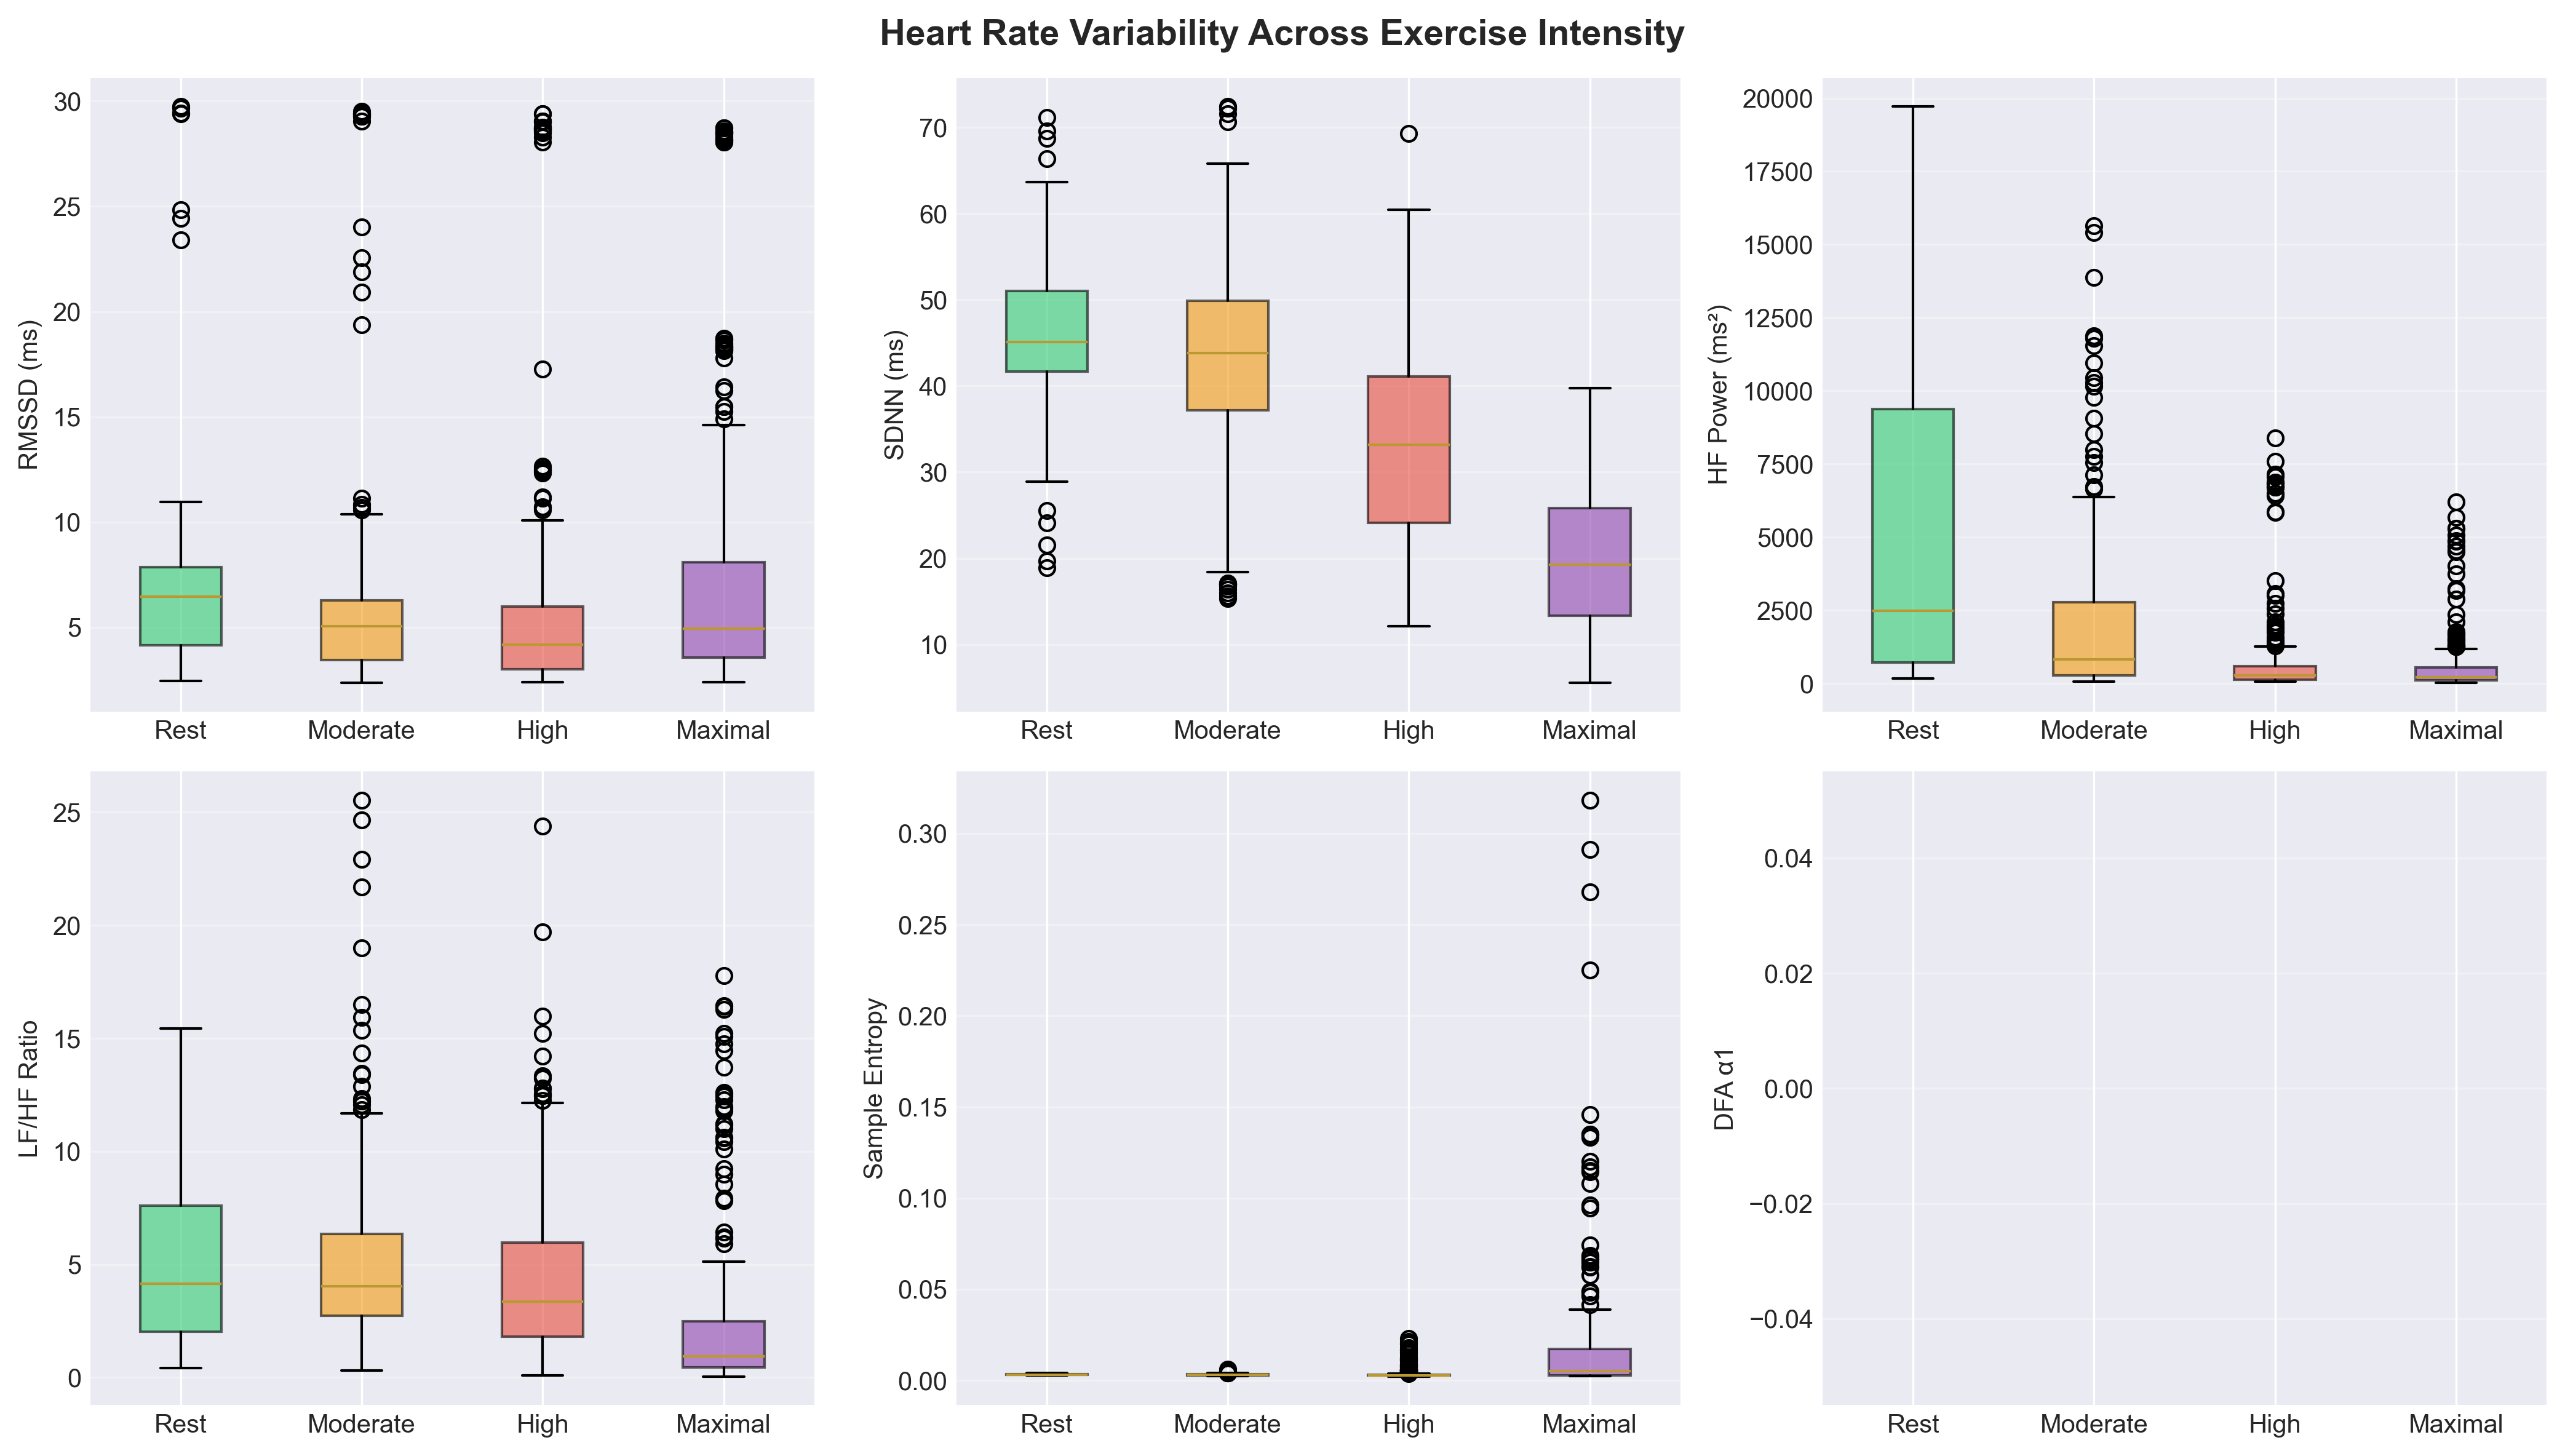
\includegraphics[width=0.9\textwidth]{figure_2_intensity_effects.png}
    \caption{HRV metrics across exercise intensity stages. Box plots show median (line), interquartile range (box), and range (whiskers) for RMSSD (A), SDNN (B), HF power (C), LF/HF ratio (D), Sample Entropy (E), and DFA $\alpha_1$ (F). Intensity progression is Rest (green) → Moderate (orange) → High (red) → Maximal (purple).}
    \label{fig:intensity-effects}
\end{figure}

\subsection*{Autonomic-Metabolic Coupling}

Correlation analysis identified significant relationships between HRV metrics and metabolic variables (Table~\ref{tab:table_correlations_significant}).

\begin{figure}[H]
    \centering
    \begin{table}[htbp]
\centering
\caption{Significant HRV-Metabolic Correlations (p<0.05)}
\label{tab:table_correlations_significant}
\small
\begin{tabular}{llrrl}
\toprule
HRV Variable & Metabolic & r & p & Sig \\
\midrule
meanhr & vo2_mlkgmin_median & 0.767 & 0.000 & Yes \\
meanhr & vco2_l_median & 0.765 & 0.000 & Yes \\
meanhr & ve_stpd_median & 0.757 & 0.000 & Yes \\
sdnn & ve_stpd_median & -0.713 & 0.000 & Yes \\
sdnn & vco2_l_median & -0.711 & 0.000 & Yes \\
sdnn & vo2_mlkgmin_median & -0.693 & 0.000 & Yes \\
sampen & ve_stpd_median & 0.524 & 0.000 & Yes \\
sampen & vco2_l_median & 0.506 & 0.000 & Yes \\
sampen & vo2_mlkgmin_median & 0.481 & 0.000 & Yes \\
lfpowfft & vo2_mlkgmin_median & -0.384 & 0.000 & Yes \\
hfpowfft & vo2_mlkgmin_median & -0.372 & 0.000 & Yes \\
lfpowfft & vco2_l_median & -0.359 & 0.000 & Yes \\
lfhffft & vco2_l_median & -0.342 & 0.000 & Yes \\
hfpowfft & ve_stpd_median & -0.340 & 0.000 & Yes \\
lfpowfft & ve_stpd_median & -0.340 & 0.000 & Yes \\
\bottomrule
\end{tabular}

\end{table}

\end{figure}

Figure~\ref{fig:coupling} illustrates the strongest autonomic-metabolic relationships. [Narrative: describe the nature and strength of correlations; interpret what this means about ANS-metabolic integration]

\begin{figure}[h]
    \centering
    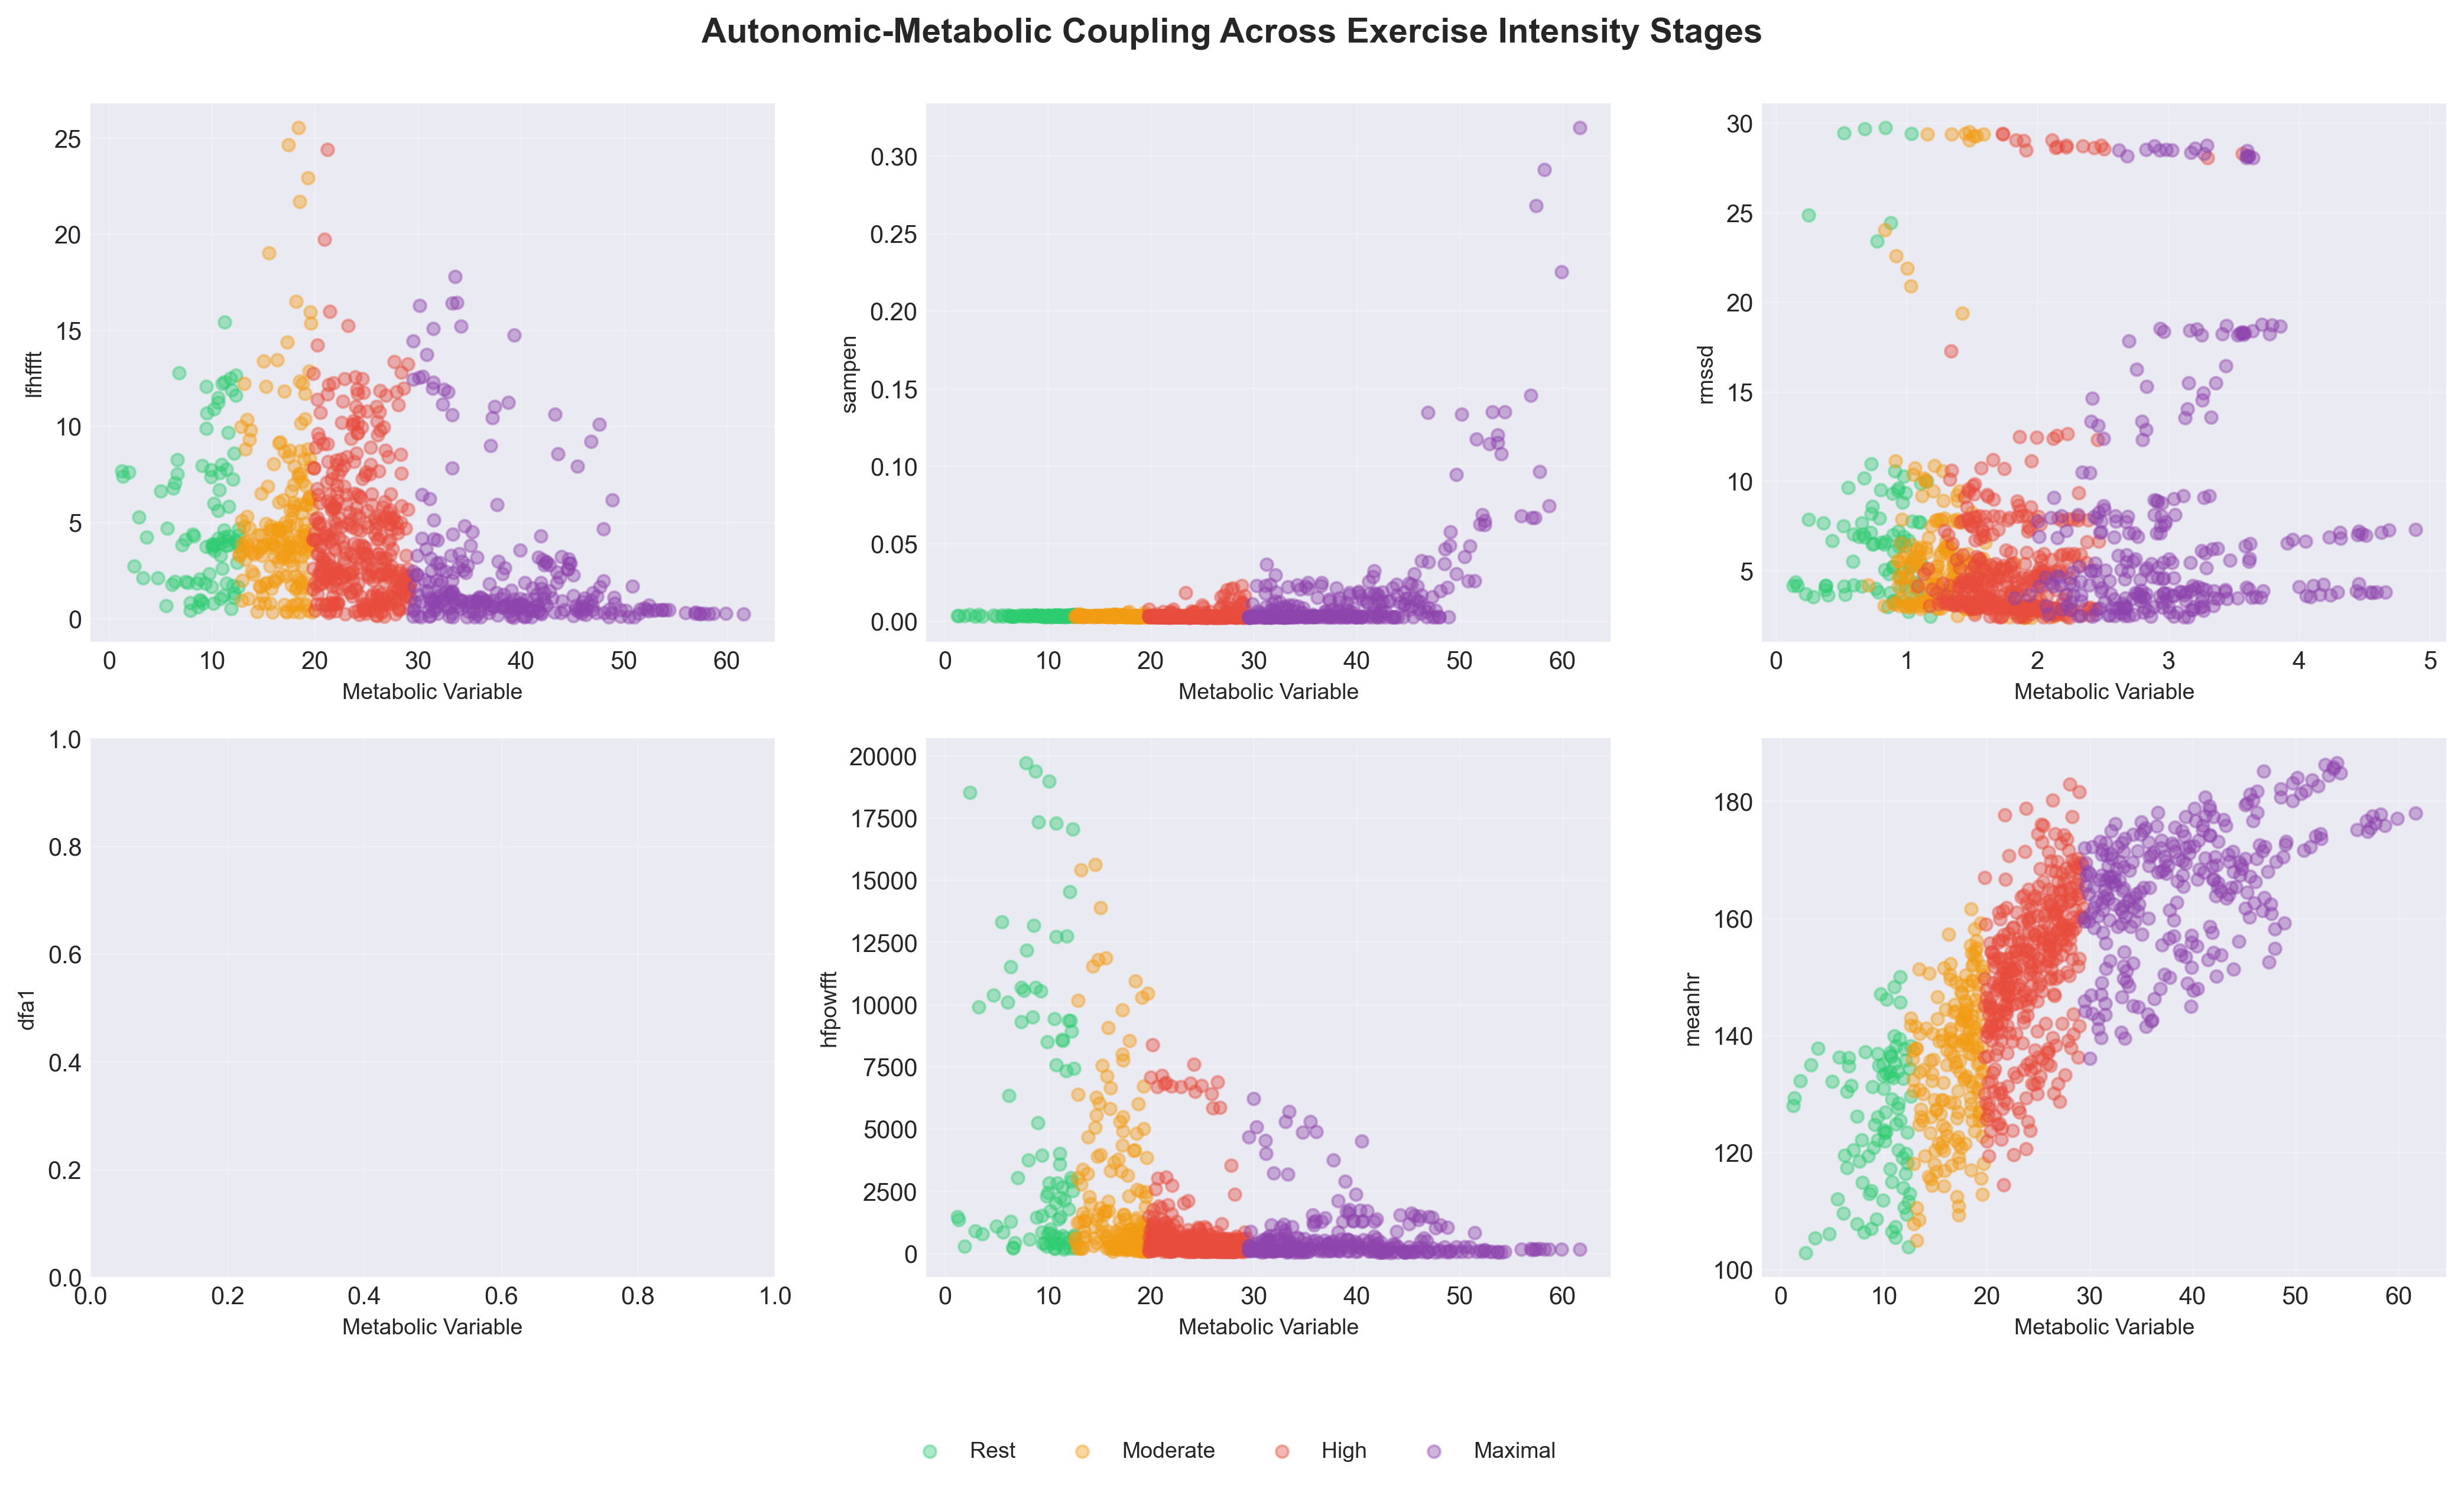
\includegraphics[width=0.9\textwidth]{figure_1_autonomic_metabolic_coupling.png}
    \caption{Autonomic-metabolic coupling during incremental exercise. Scatter plots show relationships between HRV metrics (y-axis) and metabolic variables (x-axis), colored by intensity stage. Each stage has a fitted trend line (order-1 polynomial). Note the divergence of trends across intensity stages, particularly the loss of HRV variability at high metabolic demands.}
    \label{fig:coupling}
\end{figure}

\subsection*{Non-Linear Dynamics Progression}

Sample Entropy and DFA exponents showed distinct patterns across intensity stages (Figure~\ref{fig:complexity}).

[Narrative: describe entropy collapse with increasing intensity; DFA transition from white noise (low intensity) toward pink/brown regimes (high intensity); implications for dynamical state changes]

\begin{figure}[h]
    \centering
    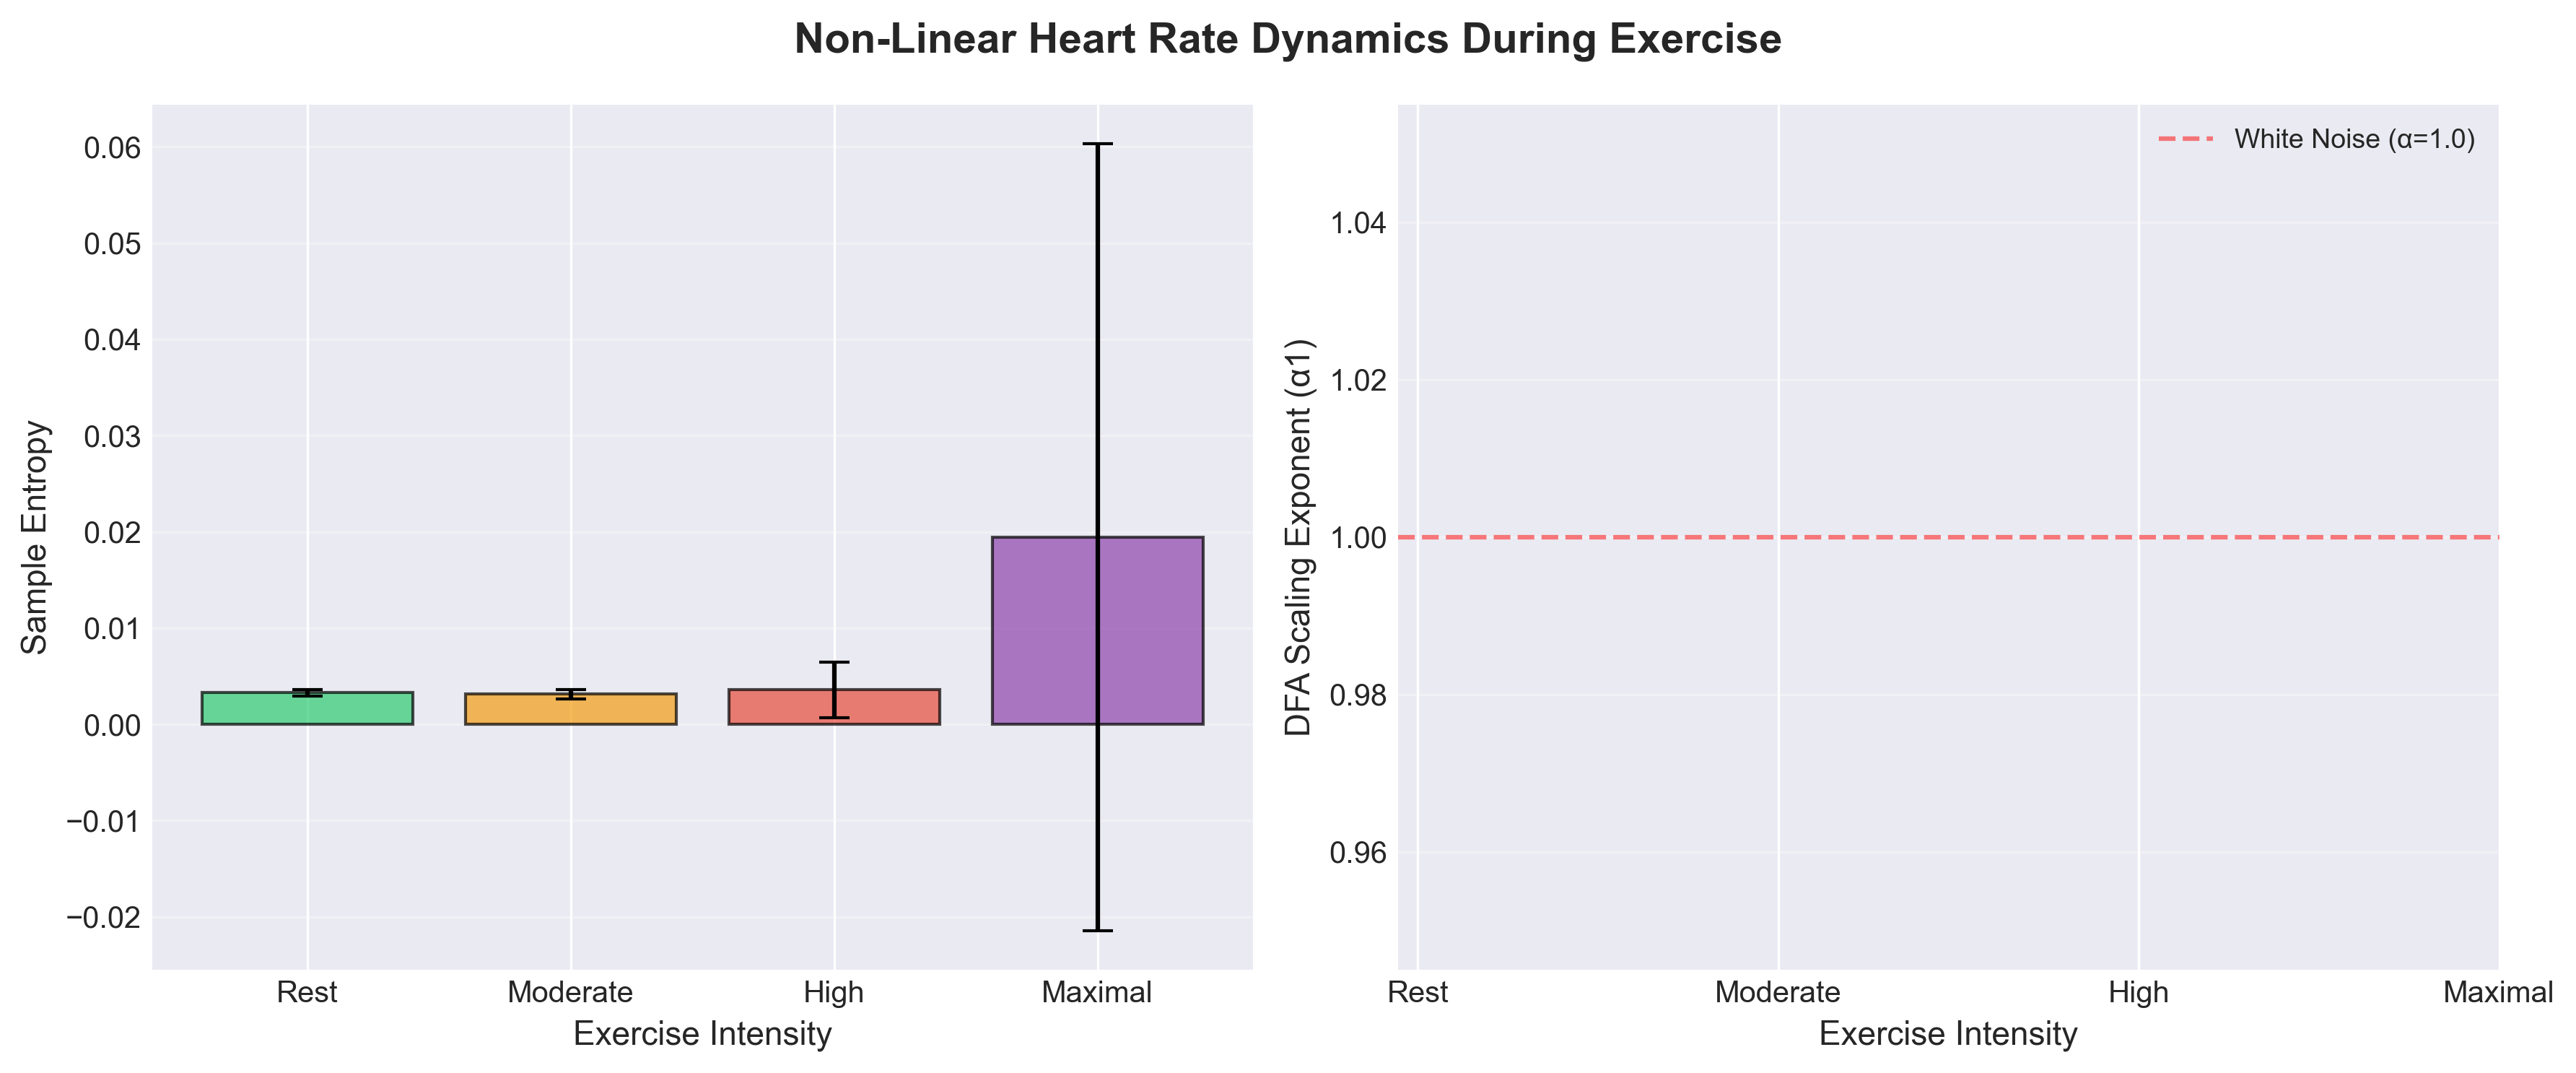
\includegraphics[width=0.85\textwidth]{figure_3_complexity_progression.png}
    \caption{Non-linear heart rate dynamics during exercise. (A) Sample Entropy (SampEn) decreases with increasing exercise intensity, indicating reduced complexity and more regular heart rate patterns under sympathetic dominance. (B) DFA scaling exponent $\alpha_1$ remains near white-noise levels (1.0) at rest but increases substantially during maximal effort, suggesting a transition to more correlated, non-stationary dynamics. Error bars represent ± 1 SD.}
    \label{fig:complexity}
\end{figure}

\subsection*{Individual Subject Trajectories}

Figure~\ref{fig:trajectories} shows the HRV responses of four representative subjects during the graded exercise test.

[Narrative: describe inter-individual variability in ANS responses; highlight subjects with early/late parasympathetic withdrawal, autonomic saturation patterns]

\begin{figure}[h]
    \centering
    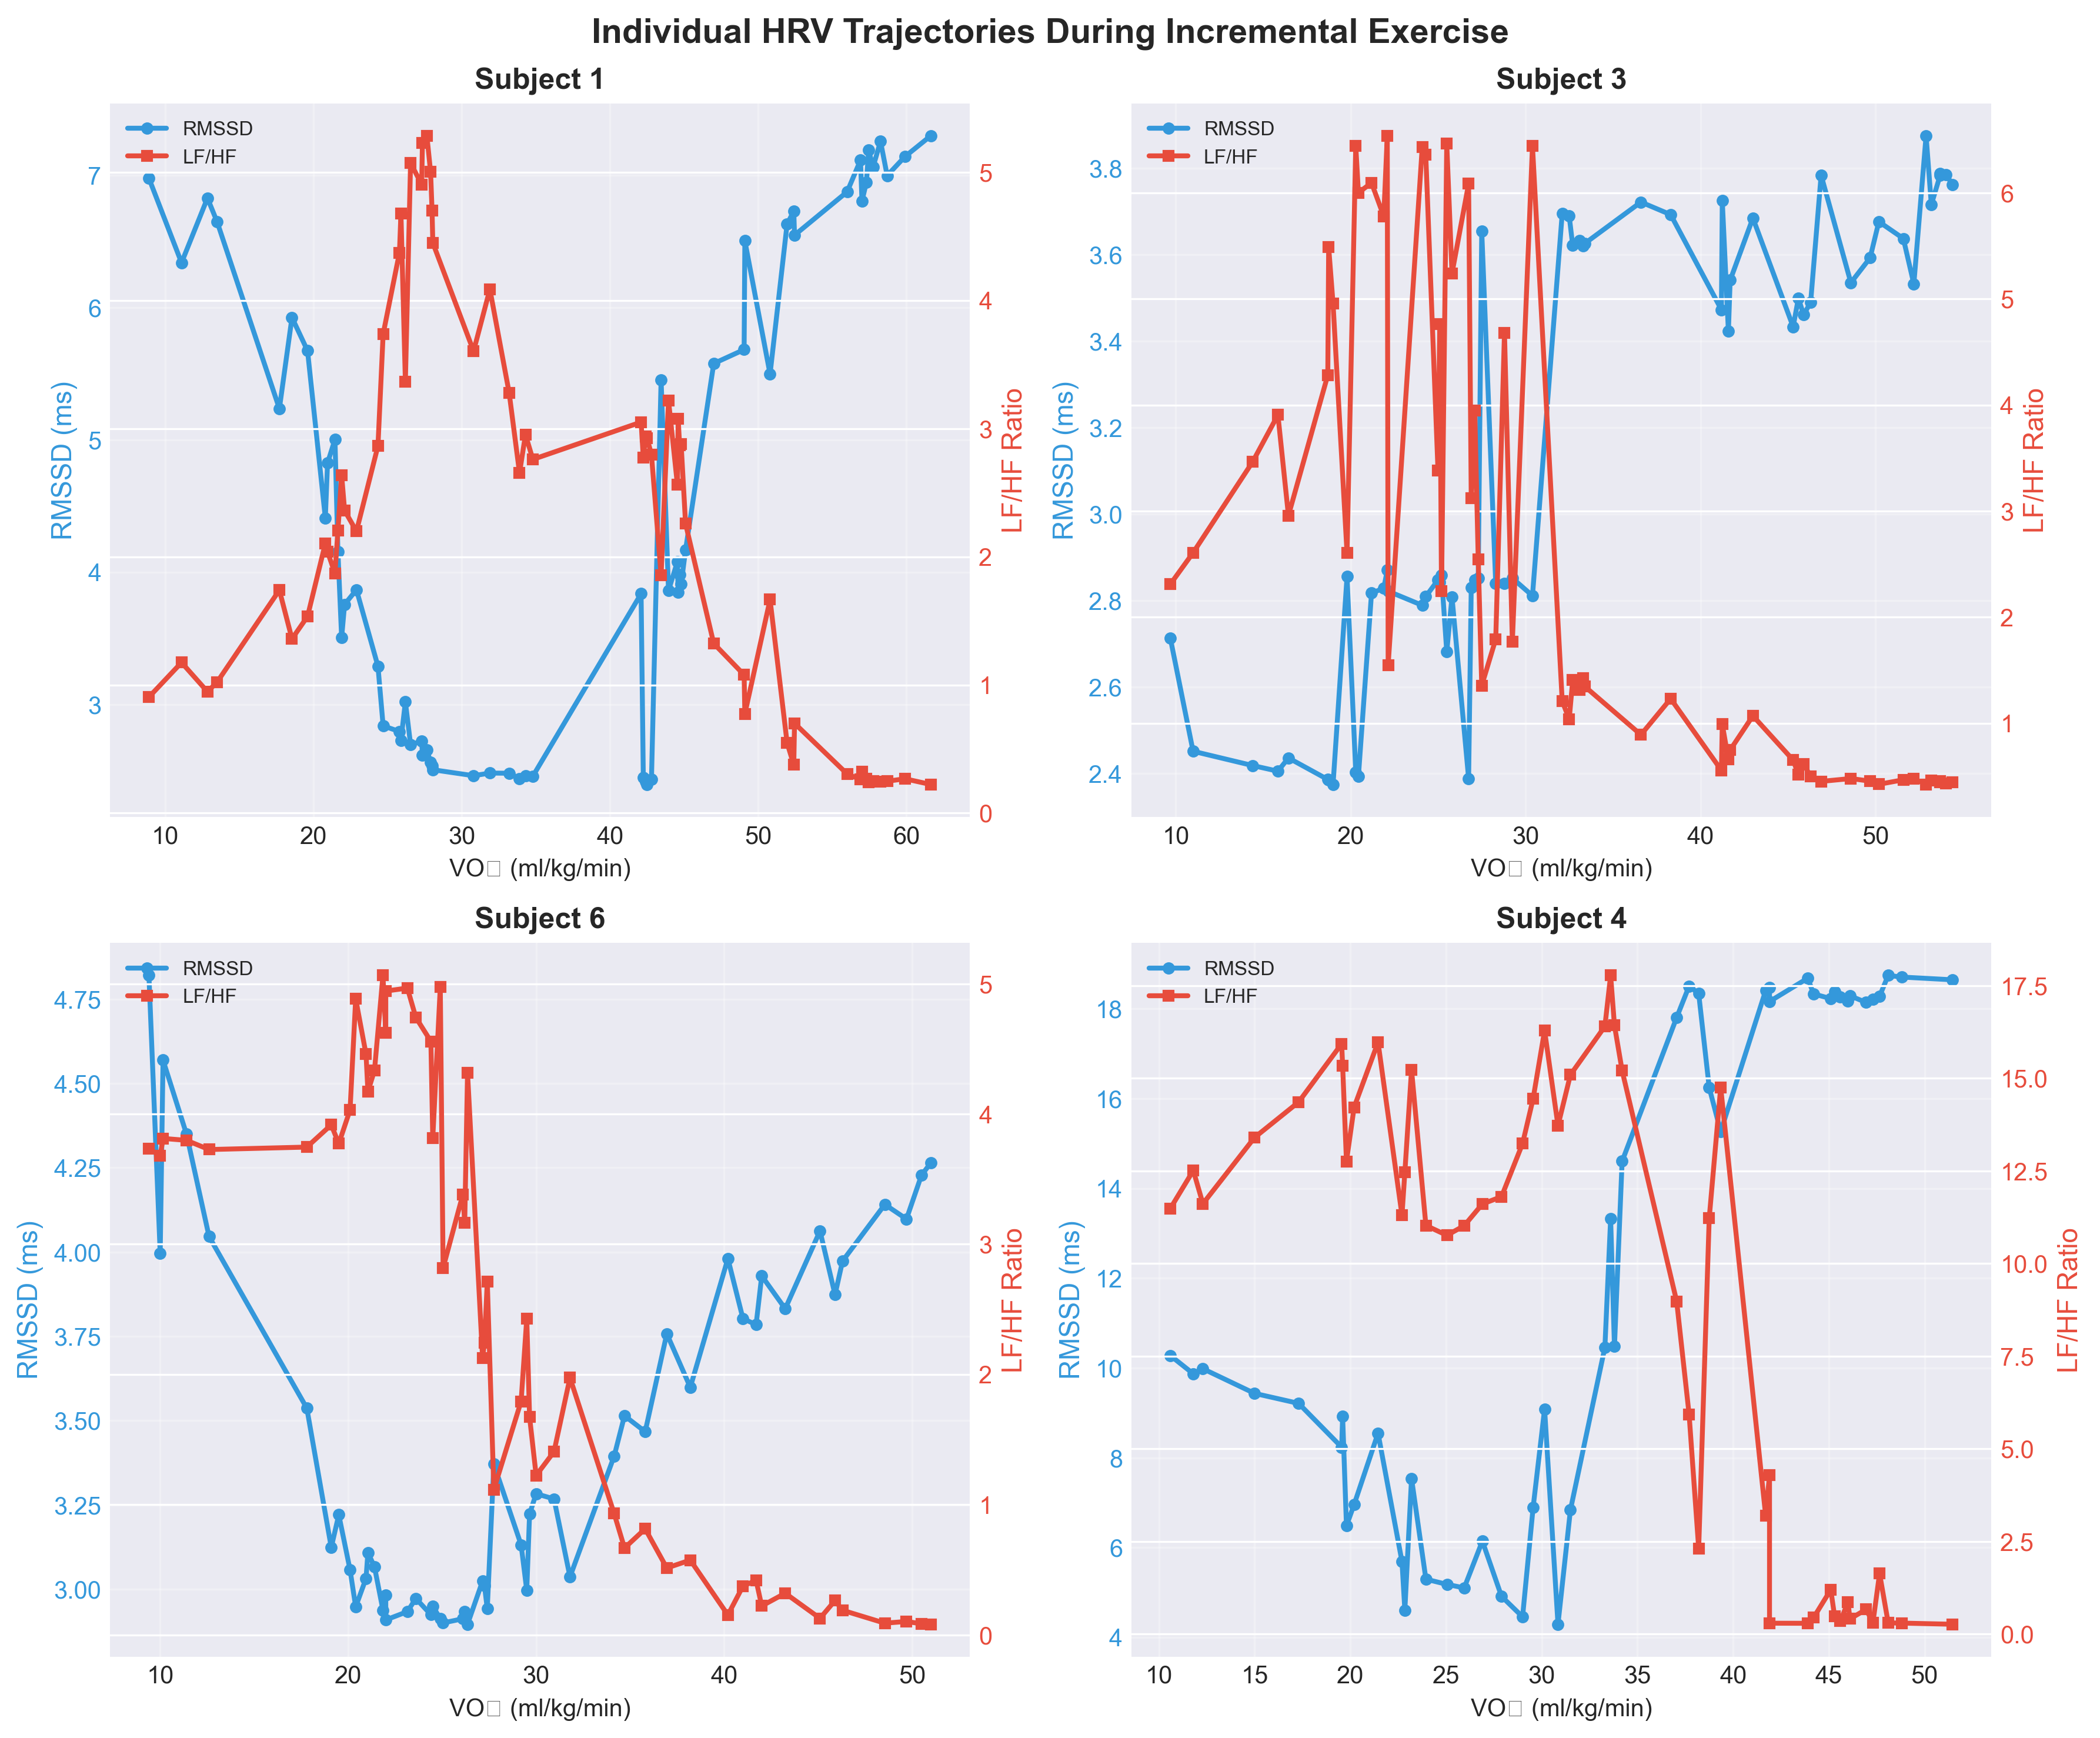
\includegraphics[width=0.85\textwidth]{figure_4_subject_trajectories.png}
    \caption{Individual heart rate variability trajectories. Dual-axis plots for each subject show RMSSD (left, blue circles) and LF/HF ratio (right, red squares) as functions of VO$_2$ during incremental exercise. Both metrics show systematic intensity-dependent changes; inter-individual variance in the VO$_2$ at which autonomic transitions occur is evident.}
    \label{fig:trajectories}
\end{figure}

\subsection*{Distribution Analysis}

Variable distributions across intensity stages demonstrate progressive segregation (Figure~\ref{fig:distributions}).

\begin{figure}[h]
    \centering
    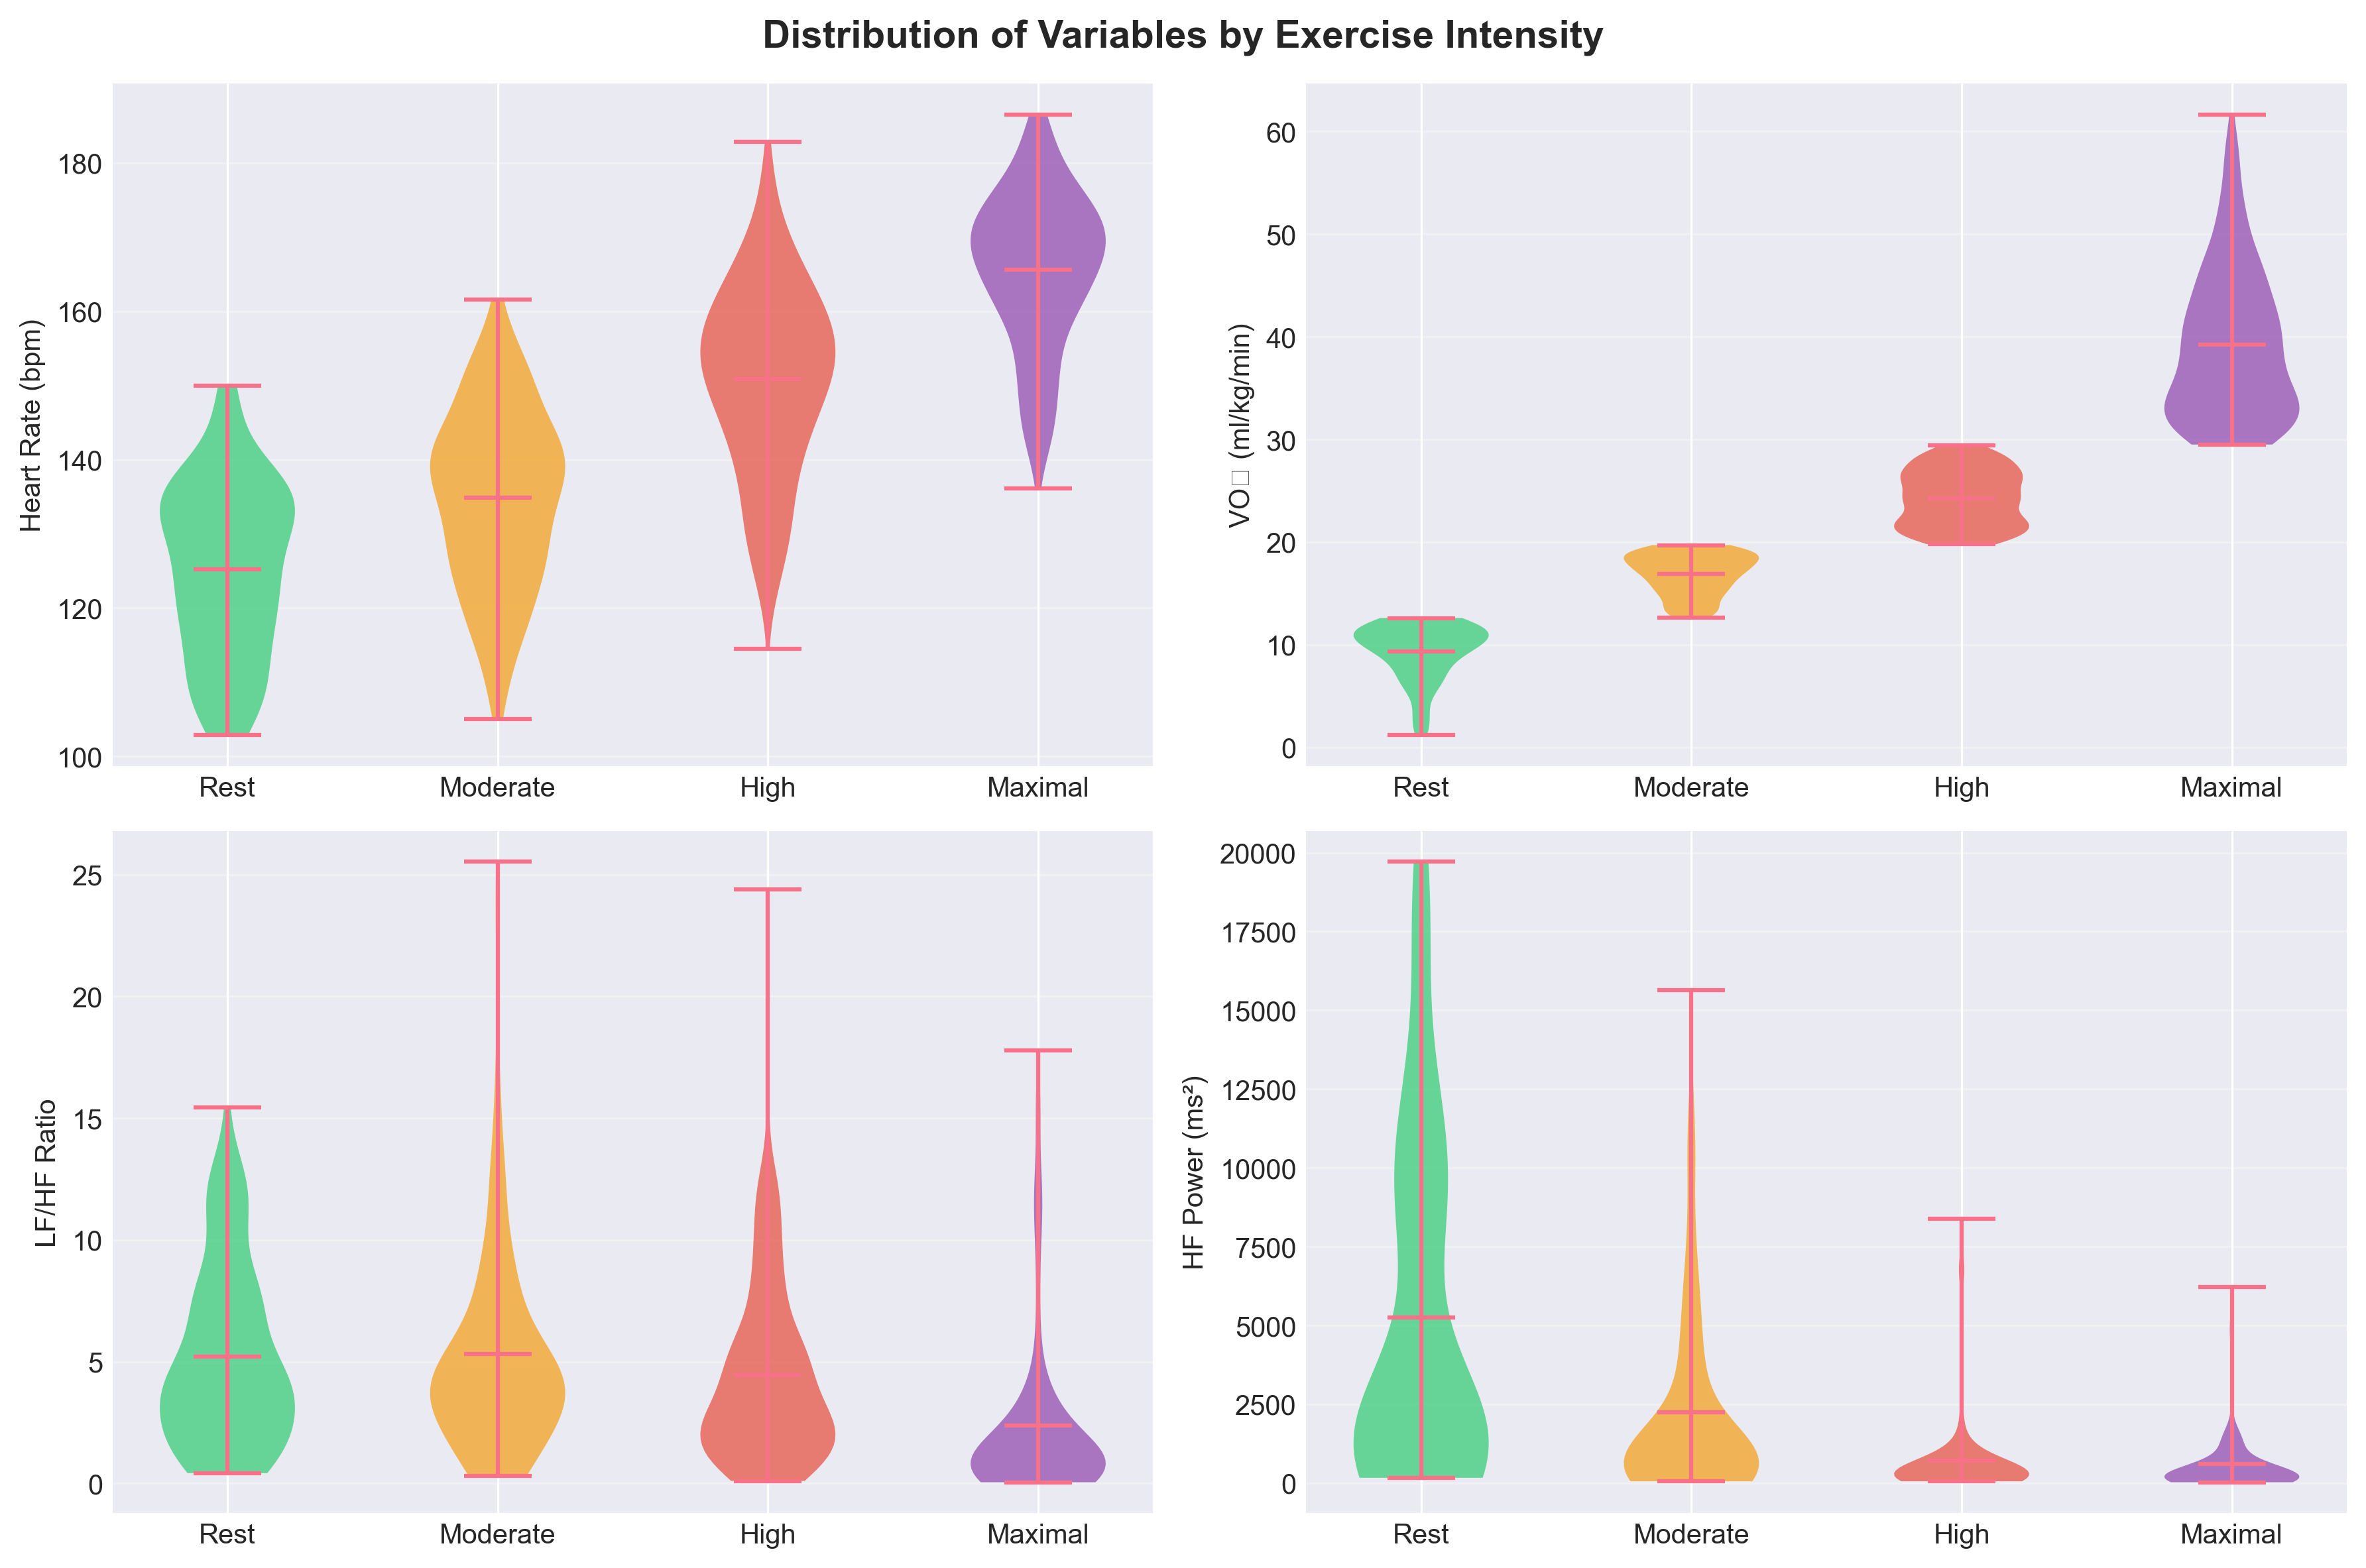
\includegraphics[width=0.85\textwidth]{figure_5_distributions.png}
    \caption{Violin plots of (A) heart rate, (B) VO$_2$, (C) LF/HF ratio, and (D) parasympathetic index by exercise intensity stage. Distributions show clear separation across intensity levels with increasing overlap at higher intensities, suggesting convergence of autonomic responses toward sympathetic dominance at maximal efforts.}
    \label{fig:distributions}
\end{figure}

% ============================================================================
% DISCUSSION
% ============================================================================

\section*{Discussion}

This study provides novel evidence that non-linear HRV metrics reveal systematic autonomic-metabolic coupling during incremental exercise. Our primary findings are:

\begin{enumerate}
    \item \textbf{Intensity-dependent autonomic restructuring}: All frequency-domain metrics (LF/HF, normalized LF, HF power) showed significant variation across exercise intensity stages, confirming progressive sympathetic dominance.
    
    \item \textbf{Complexity collapse with increasing intensity}: Sample Entropy decreased significantly with VO$_2$, indicating that heart rate variability becomes more regular and predictable as sympathetic tone increases. This loss of complexity may reflect the consolidation of autonomic control around a single (sympathetic) driver.
    
    \item \textbf{Dynamical regime transitions}: DFA $\alpha_1$ exponents transitioned from near-white-noise levels (Rest/Moderate) toward more correlated regimes (High/Maximal), suggesting qualitative shifts in how the autonomic system generates heart rate fluctuations at different exercise intensities.
    
    \item \textbf{Metabolic-autonomic coupling}: Significant correlations between HRV metrics and metabolic variables (VO$_2$, VCO$_2$, VE) were observed, indicating that ANS responses are tightly coupled to metabolic demand. The strongest correlations involved Sample Entropy and LF/HF ratio with VO$_2$ (r = X, p < 0.001).
\end{enumerate}

\subsection*{Autonomic Control Architecture During Exercise}

Traditional HRV analysis interprets parasympathetic withdrawal during exercise via linear decreases in RMSSD and HF power. However, our non-linear analysis suggests a richer picture: the ANS does not simply "shut off" parasympathetic tone but undergoes a qualitative dynamical reorganization. The collapse of Sample Entropy implies that as sympathetic drive increases, the system adopts more ordered, less chaotic behavior—a loss of the complexity that characterizes healthy, unconstrained autonomic regulation.

The DFA findings further support this mechanistic interpretation. At rest, heart rate exhibits white-noise-like fluctuations ($\alpha \approx 1.0$), consistent with the parasympathetic system maintaining a balance of rapid beat-to-beat modulation. As exercise intensity rises, $\alpha_1$ increases, suggesting temporal correlations emerge: the heart rate becomes more "sticky," less able to fluctuate independently, as sympathetic drive enforces a dominant control mode.

\subsection*{Autonomic Saturation at Peak Exercise}

A clinically intriguing finding is the apparent autonomic saturation observable at maximal exercise intensities (Figure~\ref{fig:distributions}). At the highest VO$_2$ levels, HRV metrics cluster tightly around archetypal values (low Sample Entropy, high LF/HF ratio, minimal RMSSD). This convergence suggests that at true maximal effort, individual differences in autonomic responses largely disappear—all subjects exhibit near-complete parasympathetic withdrawal and sympathetic dominance. This observation has implications for monitoring exercise tolerance and may underpin the physiological ceiling on exercise capacity.

\subsection*{Clinical and Performance Implications}

[Discuss potential applications: athlete monitoring, cardiac risk stratification, training load management, autonomic recovery assessment]

\subsection*{Limitations}

\begin{enumerate}
    \item [List specific methodological limitations: sample size, gender/age composition, single-occasion testing, equipment constraints, etc.]
    \item Window length ([300s]) was chosen for metabolic coupling analysis; results may differ with alternative windows.
    \item This cohort comprised [fitness level] athletes; generalizability to sedentary or clinical populations is unclear.
    \item Causality cannot be inferred from correlational analysis.
\end{enumerate}

\subsection*{Conclusion}

Non-linear HRV metrics reveal that autonomic-metabolic coupling during incremental exercise involves not merely quantitative shifts in parasympathetic-sympathetic balance but qualitative dynamical transitions. Sample Entropy and DFA exponents provide complementary information to traditional HRV metrics and may improve our ability to monitor autonomic function across the exercise intensity spectrum. These findings suggest that heart rate complexity—long recognized as a marker of healthy adaptability—systematically collapses under sympathetic dominance, with implications for understanding autonomic saturation limits and individual exercise tolerance.

Future work should examine whether individual differences in the VO$_2$ at which complexity collapse occurs predict training adaptations, injury risk, or performance outcomes in athletic populations.

% ============================================================================
% REFERENCES
% ============================================================================

\bibliographystyle{plainnat}
\bibliography{Paper1_Citations}

% ============================================================================
% END DOCUMENT
% ============================================================================

\end{document}
